\chapter{Arquitectura de la solución}

\textcolor{red}{En este capítulo vamos a describir los fundamentos de la arquitectura que hemos diseñado para este sistema. Comenzaremos dando una definición de las arquitecturas de \textit{software} y sus elementos. Después describiremos la arquitectura de la solución.}

\section{Arquitecturas de \textit{software}}

Según \cite{taylorSoftwareArchitectureFoundations2009}, la {\bf arquitectura de un sistema \textit{software}} es el conjunto de todas las \textbf{decisiones principales de diseño} que se toman durante su ciclo de vida; aquellas que sientan las bases del sistema. Estas afectan a todos sus apartados: la funcionalidad que debe ofrecer, la tecnología para su implementación, cómo se desplegará, etc. En conjunto, definen una pauta que guía (y a la vez refleja) el diseño, la implementación, la operación y la evolución del sistema.

\textcolor{red}{Podemos utilizarla de referencia para conocer detalles su estructura, su implementación\dots Se podría establecer un símil con los planos de construcción de un edificio. Nos provee de un marco de referencia común, de decisiones que nos nos provee con un vocabulario común, que nos permite describir sistemas}

La principal función de una buena arquitectura es dotar de estructura a nuestro sistema. \cite{martinCleanArchitectureCraftsman2018} Una buena arquitectura nos ofrece una serie de ventajas, como facilitar su desarrollo, mayor extensibilidad. Por tanto, es vital dedicar tiempo para definirla atendiendo a las necesidades de nuestro sistema.

\subsection{Decisiones principales de diseño}

Las decisiones principales de diseño son todas aquellas decisiones importantes que afectan a los fundamentos de nuestro sistema. Tienen gran importancia porque con el paso del tiempo, y con el avance del desarrollo, estas elecciones comienzan a asentarse, y se vuelven más difíciles de cambiar o rectificar. \cite{taylorSoftwareArchitectureFoundations2009} Estas no solo se toman durante la concepción del sistema, si no que también pueden surgir durante el desarrollo y posterior evolución.

Por ejemplo, una decisión de diseño principal que se suele tomar en las fases tempranas del desarrollo es la elección de la topología para la solución. Optar entre desarrollar un servicio monolítico, o un sistema formado por microservicios, va a condicionar prácticamente todo el desarrollo.

\textcolor{red}{Las decisiones principales de diseño normalmente se resumen en comparativas entre distintas alternativas, cada una de ellas con sus ventajas e inconvenientes.} Pueden tomarse en base a distintos criterios. Entre ellos podemos destacar: \textcolor{red}{[Citation needed]}

    \begin{itemize}
        \item \textbf{Requisitos del sistema:} a partir del dominio y las necesidades de nuestros usuarios, podemos deducir: la funcionalidad a implementar, las restricciones que debemos respetar y otras propiedades que debe poseer el sistema.

        \item \textbf{Arquitectura actual:} las decisiones tomadas previamente también condicionan las elecciones que se tomen más adelante. Cuanto más avanza el desarrollo, más se asientan las decisiones previas, y más dificil es rectificarlas.

        \item \textbf{Experiencia previa:} del desarrollo de este u otros sistemas. Podemos obtener métricas del funcionamiento y uso de nuestro sistema para informar decisiones futuras. \textcolor{red}{[Cita devops]}
    \end{itemize}

\subsection{Estilos arquitectónicos}

\textcolor{red}{Este conjunto de decisiones principales Una decisión de diseño principal que se suele tomar en las fases tempranas del desarrollo es la elección de un \textbf{estilo arquitectónico} para la solución. Se trata de una serie de decisiones de diseño prinEstos imponen una serie de restricciones en cuanto a la implementación del sistema, pero a su vez nos aporta una serie de beneficios... Optar por desarrollar un servicio monolítico o una arquitectura basada en microservicios va a condicionar prácticamente todo el desarrollo. Desde el diseño, la implementación, el testeo, y sobre todo, el despliegue y operación.}

\subsection{Componentes de una arquitectura}

Otra posible definición de arquitectura la encontramos en el estándar IEEE 42010-2011 \cite{ieeeStandard420102011Systems2011}: es "\textit{un conjunto de conceptos o propiedades fundamentales, personificados por sus elementos, sus relaciones, y los principios que guían su diseño y evolución}".

Podemos describirlas usando tres conceptos: \cite{perryFoundationsStudySoftware1992}

    \begin{itemize}
        \item \textbf{Elementos}: Son las piezas fundamentales que conforman el sistema. Implementan la funcionalidad de la aplicación. Se utilizan para describir \textit{qué} partes componen el sistema. Por ejemplo: un módulo, un servicio web...

        \item \textbf{Forma}: El conjunto de propiedades y relaciones entre los elementos o el entorno de operación. Describe \textit{cómo} está organizado el sistema. Por ejemplo: un servicio contacta con otro a través de una API.

        \item \textbf{Justificación}: Razonamiento o motivación de las decisiones que se han tomado. Responden al \textit{por qué} algo se hace de determinada forma. Normalmente no pueden deducirse a partir de los elementos y la forma, por lo que es necesario describirlos.

    \end{itemize}

\subsubsection{Elementos}

\textcolor{red}{La arquitectura de un sistema puede contar con diferentes vistas, según aquel aspecto que deseemos resaltar. Por ejemplo, puede interesarnos más la interacción entre los componentes. O cosas por el estilo.}

Durante el diseño del sistema, para lidiar con la complejidad que pudiera alcanzar, recurrimos a dos \textcolor{red}{mecanismos}: la abstracción y la separación de responsabilidades. \cite{martinCleanArchitectureCraftsman2018} Aplicándolas repetidamente sobre los requisitos pueden sernos de gran ayuda para identificar distintas unidades de funcionalidad. Se trata de los componentes.

Según \cite{taylorSoftwareArchitectureFoundations2009}, los \textbf{componentes} son ``elementos arquitectónicos que encapsulan un subconjunto de la funcionalidad y/o de los datos del sistema``.
Dependiendo de las características de nuestro sistema (y del nivel de abstracción que usemos) pueden tomar distintas formas: módulos dentro un mismo proceso, servicios distribuidos, etc.

\begin{wrapfigure}{r}{0.40\linewidth}
  \centering
  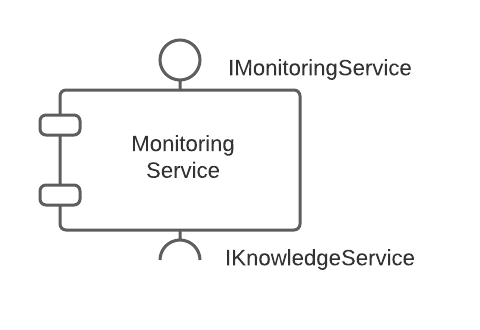
\includegraphics[scale=0.8]{02_arquitectura/images/componente-ejemplo}
  \caption{El servicio de monitorización representado como un componente. Ofrece una interfaz (\textit{IMonitoringService}) y requiere de otra para funcionar (\textit{IKnowledgeService}).}
  \label{fig:componenteEjemplo}
\end{wrapfigure}

Los componentes exponen una interfaz que permite acceso a esa funcionalidad o datos que encapsulan. A su vez, también declaran una serie de requisitos con otras interfaces de las que dependen para operar. En la figura \ref{fig:componenteEjemplo} tenemos un ejemplo.

Por si solos, estos componentes independientes no aportan mucho valor. Son la unidad básica de composición: podemos conectar distintos componentes para que trabajen conjuntamente y realicen tareas más complejas. De esta forma podemos componer sistemas. Por ello, un aspecto clave es la integración y la interacción entre componentes. \cite{mehtaTaxonomySoftwareConnectors2000}

Para que dos o más componentes puedan interactuar, necesitamos definir un mecanismo de comunicación. Recurrimos entonces a los \textbf{conectores}: se trata de elementos arquitectónicos que nos ayudan a definir y razonar sobre la comunicación entre componentes. Representan la transferencia de datos y de control entre componentes. En la figura \ref{fig:componentesYConectorEjemplo} mostramos una representación de la necesidad de comunicación entre dos componentes a través de un conector. No se ha especificado todavía ningún detalle sobre cómo se implementará. De esta forma, podemos estudiar la arquitectura y elegir los mecanismos adecuados para cada interacción del sistema. \cite{taylorSoftwareArchitectureFoundations2009}.

%% TODO: Los conectores son application-independent. No dependen de la funcionalidad de la aplicación.
%% TODO: Hablar de la cardinalidad de los conectores.

\begin{figure}[h!]
  \centering
  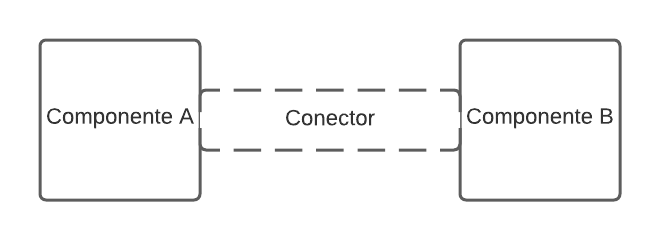
\includegraphics[scale=0.78]{02_arquitectura/images/conector}
  \caption{Ejemplo de comunicación de dos componentes a través de un conector.}
  \label{fig:componentesYConectorEjemplo}
\end{figure}

\textcolor{red}{A nivel de ¿diseño?}, los conectores están compuestos por uno o más \textbf{conductos} o canales de comunicación. A través de estos se lleva a cabo la comunicación entre los componentes. Hay una gran variedad de conductos posibles: comunicación interproceso, a través de la red, etc. Clasificamos los conectores según la complejidad de los canales que utilizan \cite{mehtaTaxonomySoftwareConnectors2000}:

\begin{itemize}
    \item \textbf{Conectores simples}: solo cuentan con un conducto, sin lógica asociada. Son conectores sencillos. Suelen estar ya implementados en los lenguajes de programación. Por ejemplo: una llamada a función en un programa o el sistema de entrada / salida de ficheros.

    \item \textbf{Conectores complejos}: cuentan con uno o más conductos. Se definen por composición a partir de múltiples conectores simples. Además, pueden contar con funcionalidad para manejar el flujo de datos y/o control. Suelen utilizarse importando \textit{frameworks} o librerias. Por ejemplo: un balanceador de carga que redirige peticiones a los nodos.
\end{itemize}

Por tanto, una vez hemos decidido que dos componentes deben comunicarse, es momento de evaluar cuál es el mecanismo de comunicación más adecuado. Para ello, podemos consultar la taxonomía de conectores de \cite{mehtaTaxonomySoftwareConnectors2000}. Basándonos en nuestros requisitos, la arquitectura ya definida, y los mecanismos de despliegue que queremos usar, elegimos el conector más adecuado.

\subsubsection{Forma}

\textcolor{red}{TODO}

\subsubsection{Justificación}

Una vez definidos los componentes y los conectores, tendremos una representación del sistema. Pero se trata de una imagen incompleta. No cuenta con ciertos detalles que nos ayudan a entenderlo mejor, como las alternativas que se consideraron en el diseño y por qué se descartaron en favor de la elegida, entre otros. Tampoco cuenta con detalles minuciosos que pueden guiar a la implementación.

Es decir, necesitamos de un concepto adicional en nuestra arquitectura para describirlos. Se trata de la \textbf{justificación}. \cite{perryFoundationsStudySoftware1992} Nos aporta detalles más precisos sobre la arquitectura.

\section{Arquitectura de la solución}

Como comentamos en el \autoref{chap:introduccion}: \nameref{chap:introduccion}, el objetivo del trabajo es adaptar un servicio monolítico para que funcione como un sistema distribuido basado en microservicios. Se trata de un cambio arquitectonico importante. Por ello, queremos diseñar una solución ingenieril teniendo en cuenta las particularidades del sistema.

Este servicio implementa un \textbf{bucle de control}, útil para dotar a un sistema con capacidades de computación autonoma. Especificamente, sigue la arquitectura del bucle MAPE-K\cite{ArchitecturalBlueprintAutonomic2006,fonsServiciosAdaptivereadyPara2021}, que mostramos en la figura \ref{fig:bucle-mapek2}. El objetivo de partida fue separar cada uno de los componentes del bucle en microservicios independientes.  \textcolor{red}{AÑADIR IMAGEN EJEMPLO DEL BUCLE DESCOMPUESTO EN MICROSERVICIOS. BUSCAR REFERENCIAS DE LIBROS SOBRE DIVIDIR MONOLITOS.}

\begin{figure}[htb]
  \centering
  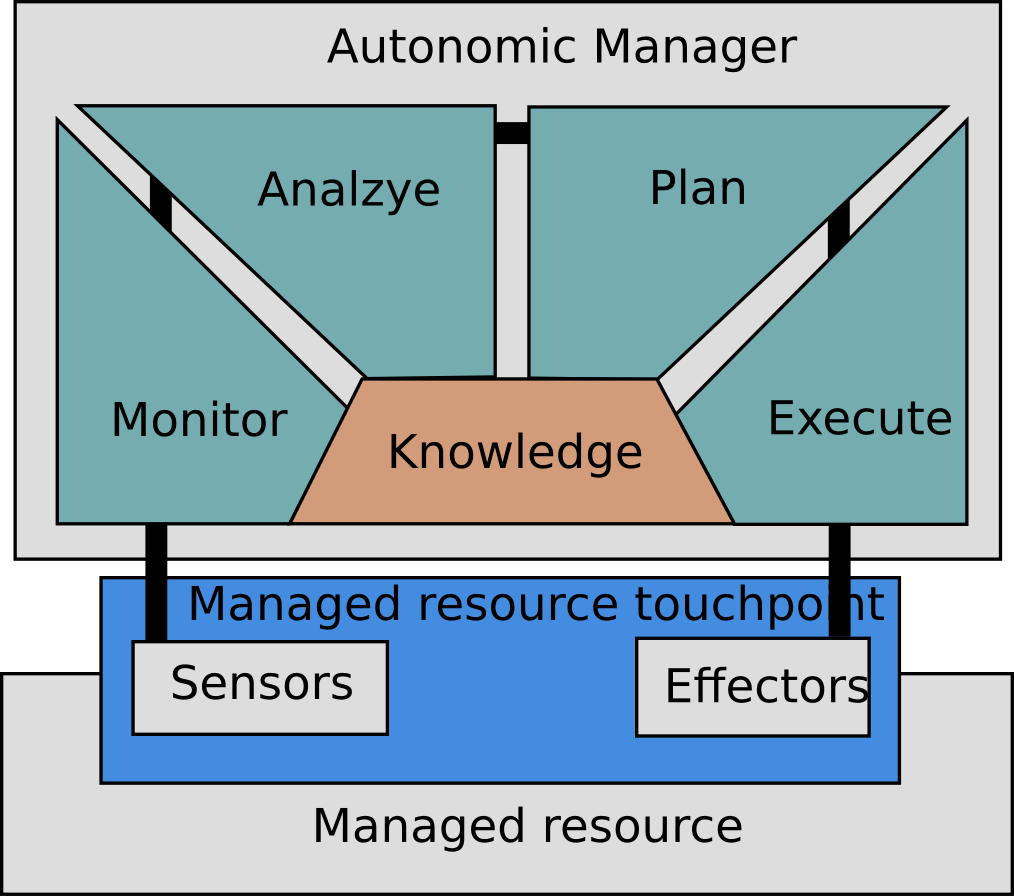
\includegraphics[scale=0.6]{01_introduccion/images/bucle-mape-k.png}
  \caption[Arquitectura de un Bucle MAPE-K.]{Arquitectura de un Bucle MAPE-K.\footnotemark}
  \label{fig:bucle-mapek2}
\end{figure}

% TODO: Cambiar por otra imagen sin typos.
\footnotetext{Obtenido de: \url{https://wwwvs.cs.hs-rm.de/vs-wiki/index.php/(WS12-01)_Cloud/Dokumentation}}

\textcolor{red}{Combinar con párrafo anterior: Actualmente, el sistema es un servicio monolitico que está muy acoplado a la solución. Queremos desacoplarlo para que pueda usarse la misma infraestructura para varios sistemas (\textit{multi-tennancy})}.

\subsection{Distribución de los componentes \textcolor{red}{TODO: MUY INCOMPLETO}}

Por suerte, partimos de un sistema existente, con una arquitectura bien definida y documentada. Conociamos el rol de los componentes del servicio y sus requisitos. Asi que, el primer problema al que nos enfrentamos estaba relacionado con la distribución de los servicios. ¿Cómo definimos las fronteras entre cada uno de ellos?

Una vez determinadas las "fronteras" entre los microservicios, hemos definido los componentes de nuestro sistema. Asi que, el primer problema al que nos enfrentamos estaba relacionado con la comunicación: si separamos las distintas etapas del bucle en microservicios, ¿cómo hacemos para que se comuniquen? Hay que tener en cuenta que estos pueden estar desplegados y replicados en distintas máquinas.

Por la descripción de ambos componentes, vemos que existe una clara división de dominios y responsabilidades. Esto nos ayuda a determinar que ambos componentes pueden desplegarse por separado. \textcolor{red}{REFERENCIA 'Building Microservices' Sam Newman}

\begin{figure}[htb]
  \centering
  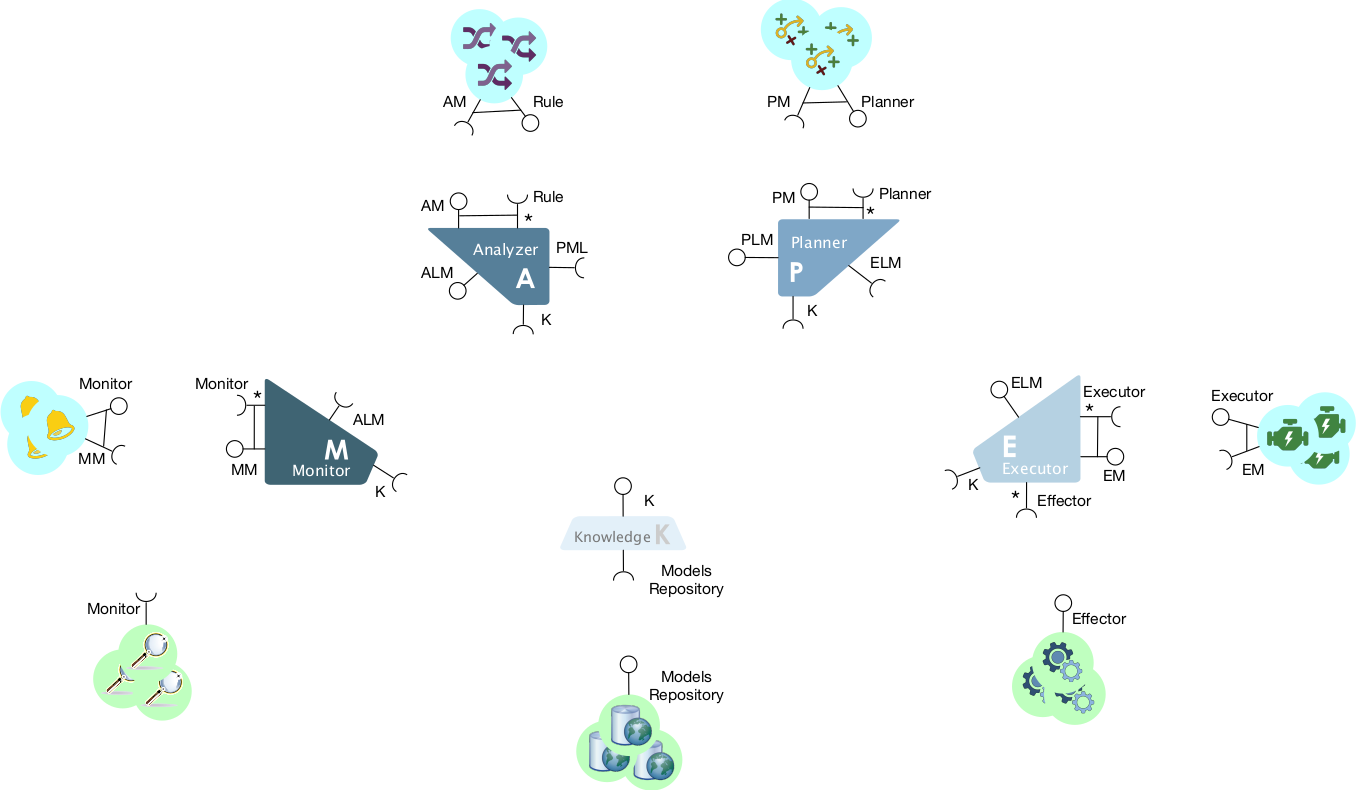
\includegraphics[scale=0.3]{02_arquitectura/images/mape-k-microservices}
  \caption{Diagrama con los componentes que forman nuestra arquitectura distribuida}
  \label{fig:mape-k-microservices}
\end{figure}

\textcolor{red}{En este caso, ponian como ejemplo un estilo arquitectónico que se llama C2 (components and connectors, creo) . La idea era tener capas o niveles de microservicios. Un microservicio en una capa concreta solo pueden contactar con sus vecinos (inmediatamente superior e inmediatamente inferior). Dentro del mismo nivel no pueden contactar entre ellos. Según la dirección de la comunicación, se utilizan mecanismos distintos:}

\begin{itemize}
  \item \textbf{Peticiones}: Un microservicio de más abajo en la jerarquía (o más externo), se comunica con un vecino que está más arriba. Por ejemplo, sería el caso de cuando el servicio de monitorización escribe una propiedad en el servicio de conocimiento.

  \item \textbf{Notificaciones}: Un microservicio de más arriba en la jerarquía (o mas interno), se comunica con un vecino que está por debajo de él. Por ejemplo, cuando el servicio de conocimiento notifica al servicio de análisis que ha cambiado una propiedad.
\end{itemize}

He encontrado una imagen que lo describe más o menos:

\begin{figure}[htb]
  \centering
  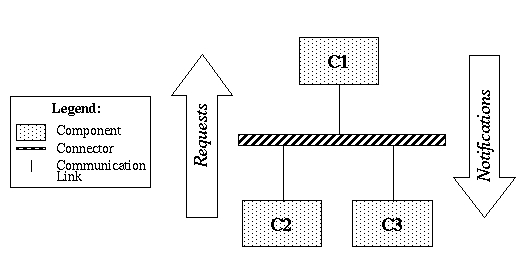
\includegraphics[scale=0.45]{02_arquitectura/images/c2SampleArch}
  \caption{Ejemplo del estilo arquitectónico C2 (\textit{Components and Connectors}). \cite{UCISoftwareArchitecture}}
  \label{fig:C2-arch-example}
\end{figure}

Mi propuesta entonces sería inspirarnos un poco en esta aproximación. Asi aprovechamos para dividir los microservicios en niveles y elegir los mecanismos para cada tipo de comunicación.

Yo distinguiría entre 4 niveles, desde más externo a más interno:

\begin{itemize}
  \item \textbf{Más externo}: Sondas y Efectores. Son los elementos que ya tienen más contacto con el sistema gestionado por el bucle. Cuanto menos esté acoplado el bucle a ellos mejor.

  \item \textbf{Nivel de solución}: En esta capa se encuentran los microservicios específicos a una solución concreta. En el ejemplo que te mostré el otro día, sería el servicio de Room Monitor, que monitoriza la temperatura de una habitación

  \item \textbf{Nivel del bucle}: Aquí se encuentran los servicios del propio bucle: servicio de monitorización, análisis, planificación y ejecución. Esta capa no debería tener dependencias con los microservicios de la solución. Es justo lo queríamos abordar en este trabajo.

  \begin{itemize}
    \item También se aprecia algo que implementé en mi solución: el servicio de monitorizacion hace de intermediario entre los monitores de la solución y el conocimiento. No se accede directamente a estas propiedades.
  \end{itemize}

  \item \textbf{Conocimiento}: Es la capa más interna y la base de la arquitectura. Todos los microservicios de la capa del bucle dependen de ella para funcionar.

\end{itemize}

Me he basado en el diagrama típico de Clean Architecture para representar un poco la idea:

\begin{figure}[htb]
  \centering
  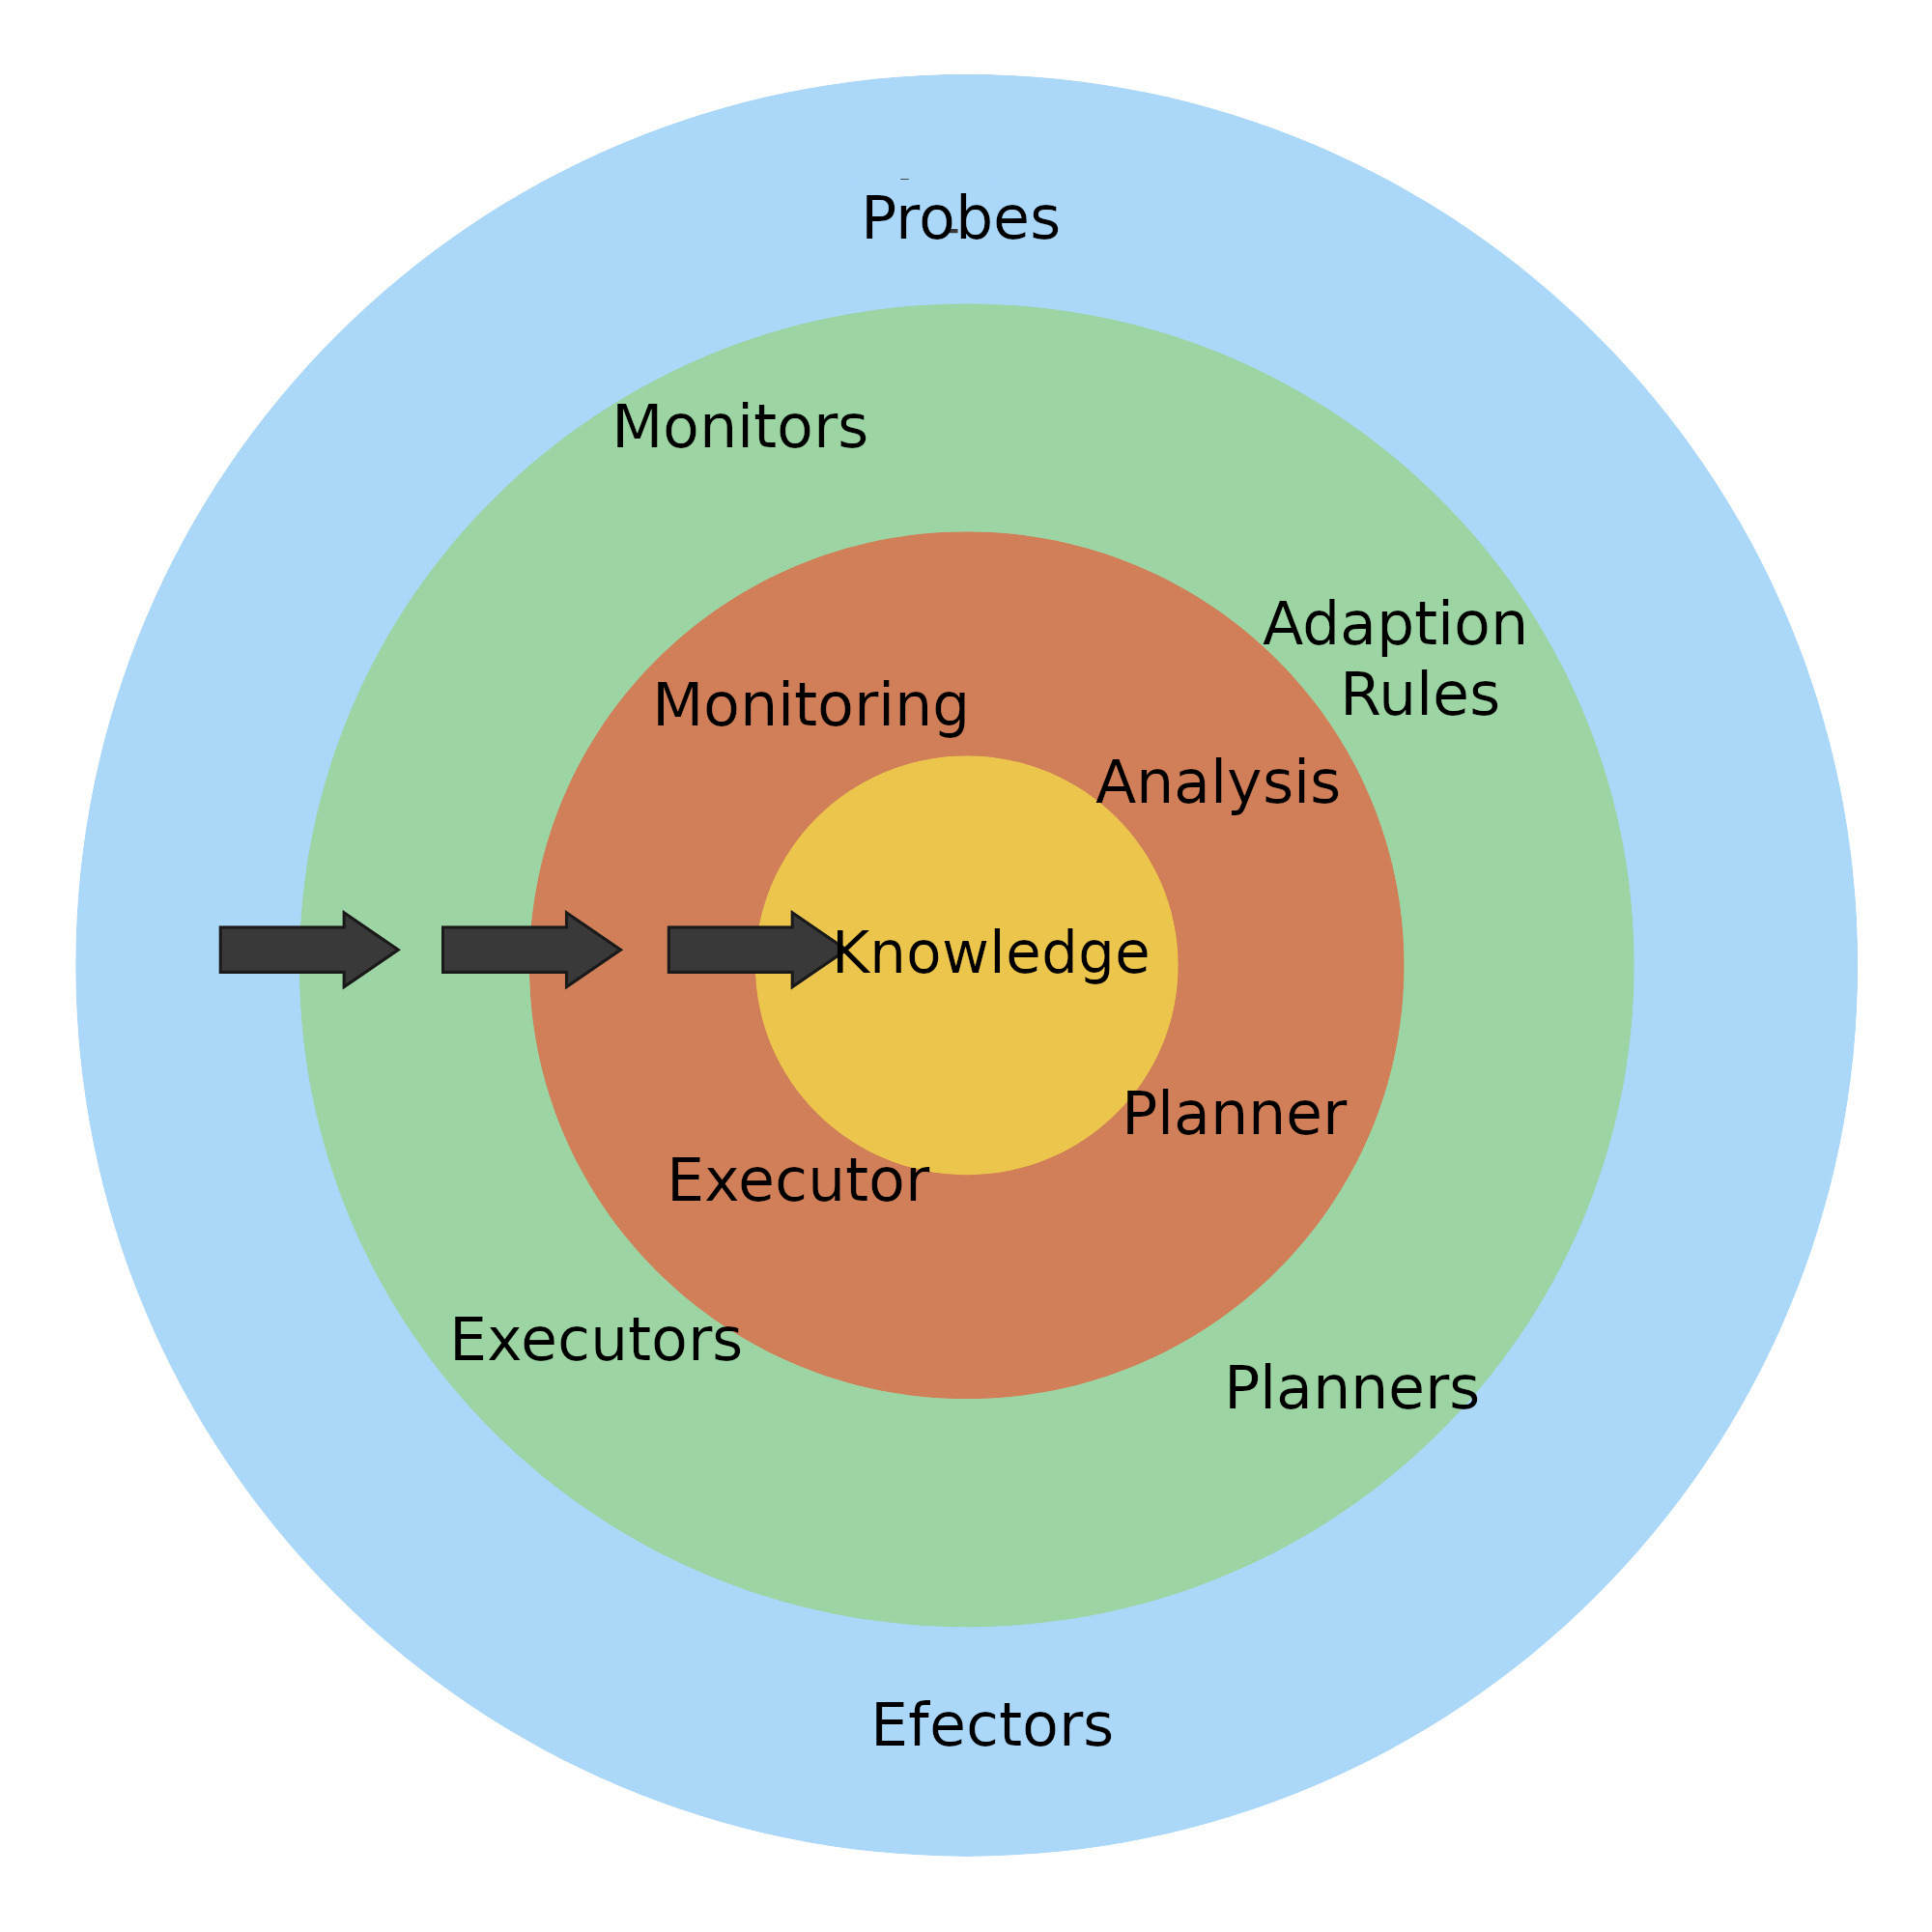
\includegraphics[scale=0.45]{02_arquitectura/images/clean-arch-2-MAPEK-style}
  \caption[Representación de nuestra propuesta arquitectónica. Inspirado en Arquitectura Limpia (\textit{Clean Architecture}).]{Representación de nuestra propuesta arquitectónica. Inspirado en Arquitectura Limpia (\textit{Clean Architecture}). \footnotemark }
  \label{fig:clean-mapek-architecture}
\end{figure}

\footnotetext{Imagen original de arquitectura limpia obtenida de: \url{https://threedots.tech/post/ddd-cqrs-clean-architecture-combined/}}


En el dibujo, las flechas de "fuera hacia adentro" representarían las Peticiones (o requests). Las notificaciones irían en sentido contrario.

Mi idea entonces es definir dos tipos de conectores:

\begin{itemize}
  \item \textbf{Peticiones}: Utilizamos la estrategia que ya definimos en el hito anterior. Los servicios ofrecen APIs REST con una serie de operaciones. Las peticiones fluyen de microservicios más externos a los más internos, mediante llamadas HTTP.

  \begin{itemize}
    \item Por ejemplo, en el hito anterior: Probe -> Monitor -> Monitoring Service -> Knowledge

    \item Utilizamos OpenAPI para autogenerar clientes, así facilitamos la implementación de los clientes en cualquier lenguaje
  \end{itemize}

  \item \textbf{Notificaciones}: En este caso optaría por usar brokers de mensajería (o algo parecido), de forma que los microservicios de capas más internos notifican a las más externas, sin necesidad de acoplarse directamente. Cada capa estaría suscrita a los eventos de la que esté por debajo de ella. Por ejemplo: Analysis Service se suscribe a Knowledge, las Reglas de Adaptación se suscriben al Analysis Service, etc.

  \begin{itemize}
    \item Seguiría un poco la filosofía que comentamos hace un tiempo para independizar el módulo de análisis del de monitorización.

    \item Podríamos investigar la idea que has comentado, de un conector que abstraiga al cliente de esta suscripción a una cola de mensajería. A esto no le he dado muchas vueltas aun.
  \end{itemize}

\end{itemize}

\subsection{Comunicación entre componentes}

Una vez determinadas las ''fronteras'' entre los microservicios, hemos definido los componentes de nuestro sistema. El siguiente problema al que nos enfrentamos fue la comunicación: si separamos las distintas etapas del bucle en microservicios, ¿cómo hacemos para que se comuniquen? Debemos tener en cuenta que estos pueden estar desplegados en máquinas distintas.

Comenzamos entonces la búsqueda de los conectores más apropiados para cada par de componentes. Seguimos la estrategia descrita en \cite{taylorSoftwareArchitectureFoundations2009} y consultando patrones de comunicación en sistemas distribuidos descritos en \cite{newmanBuildingMicroservicesDesigning2021}. \textcolor{red}{AMPLIAR} Comenzamos eligiendo qué dos componentes queremos conectar.

Tomemos por ejemplo la comunicación entre el servicio de monitorización (\textit{monitoring service}) y el servicio de conocimiento (\textit{knowledge service}). Recordemos que el servicio de conocimiento almacena todas las propiedades de adaptación. El resto de servicios necesitan consultar y actualizarlas durante su funcionamiento. En la figura \ref{fig:monitor-knowledge-initial} representamos inicialmente ambos componentes y un conector, sin especificar de qué tipo será.

% TODO: Cambiar por imagen de componentes, que ofrezcan y requieran interfaces.
\begin{figure}[htb]
  \centering
  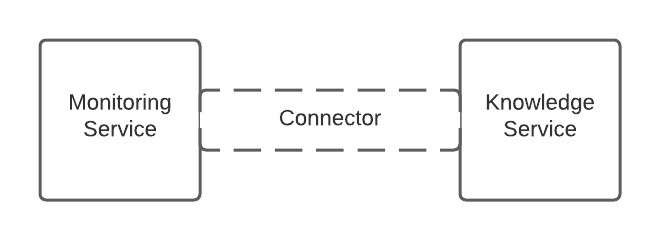
\includegraphics{02_arquitectura/images/Monitor-Knowledge-Initial-Connector}
  \caption{Boceto inicial: queremos conectar el servicio de monitorización con la base de conocimiento para poder leer propiedades de adaptación.}
  \label{fig:monitor-knowledge-initial}
\end{figure}

El siguiente paso es identificar qué interacciones debe existir entre ambos componentes. En este caso, el servicio de monitorización debe contactar con el servicio de conocimiento para leer y actualizar el valor de las propiedades. Por tanto, existen operaciones de lectura y escritura de los datos.

Ahora, debemos identificar qué \textbf{tipos de conector} serían adecuados para nuestros componentes. Sabiendo que hemos optado por una arquitectura distribuida, la elección se simplifica: los servicios pueden estar desplegados en máquinas distintas, por tanto el paso de mensajes será a través de la red.

Sabiendo esto, en lugar de recurrir a la taxonomía que lista \cite{mehtaTaxonomySoftwareConnectors2000}, optamos por consultar las estrategias de comunicación habituales para sistemas distribuidos descritas en \cite{newmanBuildingMicroservicesDesigning2021}. Se trata de cuatro mecanismos distintos: Invocación a métodos remotos (\textit{Remote Procedure Call}), APIs REST, consultas con GraphQL o \textit{brokers} de mensajería. Tuvimos que evaluarlos mediante un análisis de \textit{trade-offs} para determinar las ventajas y desventajas de cada uno.

\begin{itemize}
  \item \textbf{Invocación de métodos remotos} o (\textit{\textbf{Remote Procedure Call}}): Esta aproximación se basa en el estilo cliente-servidor. En ella, un servidor expone una serie de funciones que el cliente puede invocar mediante peticiones a través de la red. Estas peticiones incluyen el nombre de la función a ejecutar y sus parámetros. Al finalizar la ejecución, el servidor es capaz de devolver su resultado, si lo hubiera. Existen varios protocolos que implementan este mecanismo como gRPC o SOAP.

  Una evolución de RPC suele emplearse en la programación orientada a objetos: el paradigma de objetos distribuidos. \cite{tanenbaumChapter10Distributed2007} En este caso, el programa cliente interactúa con objetos que se encuentran en servidores remotos. Esta interacción se realiza a través de objetos que actúan como \textit{proxies}, abstrayendo de la llamada al servidor.

  Los \textit{proxies} ofrecen una interfaz para que el cliente invoque sus métodos localmente. Internamente, estos métodos realizan una llamada al servicio remoto donde se encuentra el objeto realmente. El servidor remoto procesa la petición y nos devolverá un resultado. Así, abstraen al cliente de todo este proceso de comunicación. En la figura \ref{fig:rpc-distributedobjects} tenemos un esquema de este mecanismo.

  \begin{figure}[htb]
    \centering
    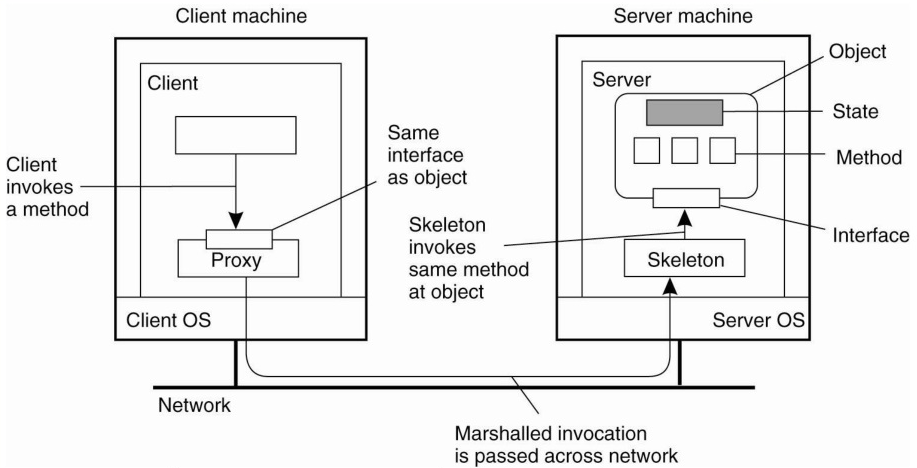
\includegraphics[scale=1.5]{02_arquitectura/images/rpc-distributedobjects}
    \caption[Funcionamiento del sistema de objetos distribuidos]{Funcionamiento del sistema de objetos distribuidos. \cite{tanenbaumChapter10Distributed2007}}
    \label{fig:rpc-distributedobjects}
  \end{figure}

  \begin{itemize}
    \item \textbf{Ventajas}:
    \begin{itemize}
      \item Permite la distribución del procesamiento del sistema.

      \item Abstrae al cliente de esta interacción con un servidor remoto. Para el cliente es prácticamente indistinguible de un objeto local.

      \item Los \textit{proxies} o (\textit{stubs} en la terminología de RPC) suelen generarse a partir de un contrato que define qué operaciones ofrecen estos objetos. Por ejemplo: SOAP con WDSL, gRPC; o en el caso de objetos distribuidos, Java RMI.
    \end{itemize}

    \item \textbf{Desventajas}:
    \begin{itemize}
      \item No se puede abstraer completamente al cliente de las llamadas a través de la red. Pueden darse errores que no ocurrirían durante una invocación de un método sobre un objeto local. Por ejemplo, que el servidor no esté disponible. \cite{jausovecFallaciesDistributedSystems2020}

      \item Dificulta la integración. Cada servicio ofrece sus propias funciones distintas.

      \item Si adoptamos sistemas como Java RMI, nuestro sistema se acopla a esa tecnología concreta. \cite{newmanBuildingMicroservicesDesigning2021}. Nos resta flexibilidad en cuanto a qué otras tecnologías podemos utilizar en nuestra arquitectura.

      \item El cliente debe actualizarse y recompilarse con cada cambio en el esquema del servidor. Esto puede ser problemático para casos donde tenemos que desplegar una actualización para que nuestros clientes puedan continuar utilizando la aplicación.
    \end{itemize}
  \end{itemize}

  \item \textbf{\textit{Representational State Transfer} (REST)}: Se basa también en el estilo arquitectónico cliente-servidor, pero con ciertas restricciones adicionales. \cite{taylorSoftwareArchitectureFoundations2009} Su concepto principal son los \textbf{recursos}: cualquier elemento del cual la API puede ofrecernos información y que pueda tener asociado un identificador único (una URI). \cite{richardsonRESTfulWebServices2007} Por ejemplo, podrían ser las entidades del dominio que gestiona nuestro servicio: Usuarios, Temperaturas\dots

  Las acciones que podemos ejecutar sobre los recursos (leer, crear, actualizar, \dots) las define el protocolo de comunicación sobre el que se implemente. Gracias a esto, la API que pueden ofrecer los servicios REST es común. Solo cambia el ``esquema de los datos``, los tipos de recursos que ofrecen. Esto facilita enormemente la integración con otros servicios. \cite{nallyRESTVsRPC2018} La implementación más común de REST es sobre el protocolo HTTP.

  \begin{itemize}
    \item \textbf{Ventajas}:

    \begin{itemize}
      \item \textbf{\textit{Stateless}}: El servidor no mantiene el estado de la sesión. Esto permite que cada petición sea independiente de las demás.

      \item \textbf{Escalable}: Como las sesiones deben ser \textit{stateless}, podremos replicar nuestro servicio y que distintas instancias puedan atender las peticiones que surjan durante la sesión.

      \item \textbf{API Sencilla}: Solo hay que implementar unos pocos métodos estándar para interactuar con la API.

      \item \textbf{Comunicación síncrona}: Es el mecanismo ideal para comunicaciones síncronas, donde el cliente requiere la respuesta del servicio para poder continuar con su procesamiento. También podemos dar soporte a para comunicaciones \textit{fire and forget}, donde el cliente envía un mensaje y no espera ninguna respuesta a su petición.

      \item \textbf{Interoperabilidad}: Ampliamente utilizado en servicios de Internet. Es ideal para que clientes externos contacten con nuestro sistema mediante peticiones síncronas. \cite{newmanBuildingMicroservicesDesigning2021}

      \item \textbf{Generación de clientes}: Para facilitar la comunicación con APIs REST, podemos generar librerias cliente utilizando el estándar OpenAPI. Lo explicaremos con maś detalle en la sección \ref{chap:OpenAPI}.
    \end{itemize}

    \item \textbf{Desventajas}:

    \begin{itemize}
      \item \textbf{Rendimiento}: El rendimiento es peor comparado con mecanismos RPC. El tamaño de un mensaje HTTP serializado en XML o JSON es mayor que si estuviera en un formato binario.

      \item \textbf{API Sencilla}: También es una desventaja. Hay operaciones complejas que es difícil representar con los métodos ofrecidos por el protocolo de comunicación. Pueden requerir más tiempo de diseño, o incluso ser implementados siguiendo RPC.
    \end{itemize}
  \end{itemize}

  \item \textbf{GraphQL}\footnote{Página oficial: \url{https://graphql.org/}} \textcolor{red}{AMPLIAR}: Se trata de un protocolo para que un cliente pueda hacer consultas personalizadas sobre los datos de un servidor. No necesitan que haya sido implementado con lógica asociada. De esta forma, se puede reducir la cantidad de peticiones a través de la red que se necesita ejecutar para obtener la misma información.

  \begin{itemize}
    \item \textbf{Ventajas}:

    \begin{itemize}
      \item \textbf{Ideal para móviles}: Gracias a que reduce la cantidad de llamadas, es ideal para entornos donde queremos optimizar el uso de datos.

      \item \textbf{Rendimiento}: Ofrece un mayor rendimiento comparado con otras alternativas que no ofrezcan un endpoint ya implementado. Y debamos obtener la misma información por composición, haciendo varias llamadas.
    \end{itemize}

    \item \textbf{Desventajas}:

    \begin{itemize}
      \item \textbf{Exponemos datos a la red}:

      \item \textbf{Problemas de rendimiento}: El cliente puede hacer consultas muy pesadas que penalicen el rendimiento de la base de datos sobre la que opera nuestro servicio.
    \end{itemize}
  \end{itemize}

  \item \textbf{\textit{Brokers} de mensajería}: Es un mecanismo de \textbf{comunicación asíncrona} muy popular. Sobre todo en arquitecturas basadas en eventos. Contamos con un servicio que actúa como intermediario, el \textit{broker}. Este gestiona la comunicación entre los servicios del sistema. \cite{newmanBuildingMicroservicesDesigning2021} Hay varias estrategias de comunicación posibles: punto a punto, \textit{publish-suscribe}, híbrida\dots

  Tomemos por ejemplo \textit{publish-suscribe}: es una estrategia para implementar comunicación \textit{multicast}. Se basa en el uso de \textbf{temas} o \textbf{\textit{topics}}, categorías de mensajes que pueden resultar de interés. Un servicio (el productor) envía un mensaje al \textit{broker}, indicando que pertenece a un tema determinado. El \textit{broker} recibe el mensaje y se encarga de reenviarlo a todos los servicios subscritos a este tema en cuanto sea posible. \cite{rabbitmqPublishSubscribeDocumentation} En la figura \ref{fig:publish-subscribe} tenemos un ejemplo de esta estrategia.

  \pagebreak

  \begin{figure}[htb]
    \centering
    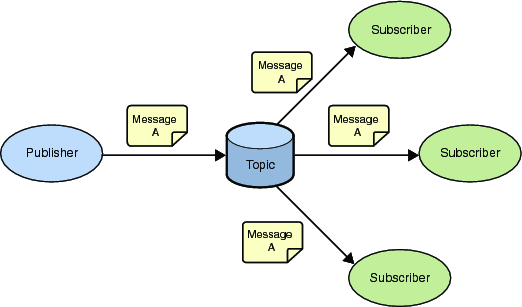
\includegraphics[scale=0.5]{02_arquitectura/images/publish_subscribe}
    \caption[Estrategia \textit{publish/suscribe}: el \textit{broker} actúa como intermediario en la comunicación \textit{multicast}.]{Estrategia \textit{publish/suscribe}: el \textit{broker} actúa como intermediario en la comunicación \textit{multicast}. Imagen obtenida de \footnotemark}
    \label{fig:publish-subscribe}
  \end{figure}

  \footnotetext{Java Messaging Service: \url{https://docs.oracle.com/cd/E19509-01/820-5892/ref_jms/index.html}}

  La mayor ventaja de este estilo de comunicación es el \textbf{desacoplamiento} entre los servicios. \cite{korabUnderstandingMessageBrokers2017}
  Ninguno de ellos necesita conocer detalles sobre cómo están desplegado los otros: su dirección, el número de instancias, si están activos en este momento, etc. Solo necesitan conocer la dirección del \textit{broker} para enviar o recibir mensajes.

  \begin{itemize}
    \item \textbf{Ventajas}:

    \begin{itemize}
      \item \textbf{Comunicación asíncrona}: El servicio no necesita quedarse a la espera de una respuesta del servidor. Puede procesar otras operaciones hasta que se le notifique del resultado, si lo hubiera.

      \item \textbf{Desacoplamiento de los servicios}: Ni los productores ni los consumidores necesitan conocer el origen o destino de sus mensajes.

      \item \textbf{Envío garantizado de mensajes}: El \textit{broker} garantiza que el mensaje será entregado \textit{al menos} una vez.

    \end{itemize}

    \item \textbf{Desventajas}:

    \begin{itemize}
      \item \textbf{Requisitos de infraestructura}: Utilizar un \textit{broker} de mensajería implica tener ciertas consideraciones a la hora de diseñar nuestro plan de despliegue. Estos sistemas requieren de replicación para alcanzar la alta disponibilidad necesaria para que sea fiable. \cite{newmanBuildingMicroservicesDesigning2021} Por tanto, aumenta la complejidad de operar el sistema.

      \item \textbf{Envío garantizado de mensajes}: Para poder garantizar el envío de un mensaje, el \textit{broker} puede recurrir a reenviarlo. Debemos diseñar nuestros sistemas de forma que estos mensajes duplicados, si ya han sido procesados, deben ser descartados.
    \end{itemize}
  \end{itemize}
\end{itemize}

De estas cuatro opciones, podemos descartar inmediatamente la opción de GraphQL. Se trata de un conector más orientado a las consultas de datos. En nuestro caso, necesitamos ejecutar también escrituras de los valores de las propiedades. Siguiendo también este razonamiento nos llevó a descartar el \textit{broker} de mensajería. Para obtener propiedades del conocimiento, resultaba más sencillo de implementar mediante comunicación síncrona.

Finalmente, hay que tener en cuenta que una de nuestras prioridades es la \textbf{interoperabilidad}: es una API expuesta ''hacia fuera'', hacia una capa más externa; prima por tanto la compatibilidad con cualquier tipo de cliente. Descartamos entonces RPC, dado que nos acoplaría a una tecnología concreta y a APIs no estándares.

Terminamos por tanto decantándonos por implementar la comunicación utilizando un conector REST sobre HTTP. Implementamos ambas funciones mediante \textit{endpoints} HTTP. Su especificación se detalla a continuación en las tablas \ref{tab:especificacion-get-property} y \ref{tab:especificacion-put-property}.

\newsavebox\getpropertyrequestbox
\begin{lrbox}{\getpropertyrequestbox}
  \begin{minipage}[t]{1in}
  \begin{verbatim}
Request:
HTTP GET property/currentTemperature

Response: 200 Ok
{
  value: {
    "Value":16.79,
    "Unit": 1, // Celsius
    "ProbeId":"c02234d3-329c-4b4d-aee0-d220dc25276b",
    "DateTime":"2022-01-15T18:19:38.5231231Z"
  },
  lastModification: "2022-01-15T18:19:39.123213Z"
}
  \end{verbatim}
  \end{minipage}
\end{lrbox}

\begin{table}[htb]
  \centering

  \begin{tabular}{|m{3.4cm}|p{2.5cm}|p{1cm}|p{3cm}|}
      \hline

      \textbf{Operación HTTP} & GET & \textbf{Ruta} & property/\{\textit{propertyName}\} \\
      \hline

      \textbf{Descripción} & \multicolumn{3}{|l|}{Devuelve el valor de la propiedad, si existe.} \\
      \hline

      \textbf{Parámetros} & \textit{propertyName} & \multicolumn{2}{|m{0.55\linewidth}|}{El nombre de la propiedad que deseamos obtener. Se lee a partir de la ruta de la petición.}\\
      \hline

      \multirow{3}*{\textbf{Respuestas posibles}}
            & \textbf{Código 200 (Ok)} & \multicolumn{2}{|m{0.55\linewidth}|}{La propiedad se ha encontrado. Incluye un \textit{payload} con el siguiente esquema:

  \begin{itemize}
              \item \textit{Value}: Valor de la propiedad serializado en JSON.
              \item \textit{LastModification}: Fecha y hora de la última modificación de esta propiedad.
            \end{itemize}}\\

            \cline{2-4}

            & \textbf{Código 400 (Bad request)} & \multicolumn{2}{|m{0.55\linewidth}|}{La petición está mal formada, no es acuerdo al contrato.}\\

            \cline{2-4}

            & \textbf{Código 404 (Not found)} & \multicolumn{2}{|m{0.55\linewidth}|}{No se ha encontrado ninguna propiedad con el nombre proporcionado.}\\
      \hline

      \textbf{Ejemplo} & \multicolumn{3}{|b{0.7\linewidth}|}{Petición para obtener la propiedad \textit{currentTemperature}:
      \usebox\getpropertyrequestbox} \\

      \hline
  \end{tabular}

  \caption{Especificación de la operación para obtener una propiedad del servicio de conocimiento.}
  \label{tab:especificacion-get-property}
\end{table}

\newsavebox\putpropertyrequestbox
\begin{lrbox}{\putpropertyrequestbox}
  \begin{minipage}[t]{2in}
  \begin{verbatim}
Request:
HTTP PUT property/currentTemperature

{
  value: {
    "Value":16.79,
    "Unit": 1, // Celsius
    "ProbeId":"c02234d3-329c-4b4d-aee0-d220dc25276b",
    "DateTime":"2022-01-15T18:19:38.5231231Z"
  }
}

Response: 204 (No content)
  \end{verbatim}
  \end{minipage}
\end{lrbox}

\begin{table}[htb]
  \centering

  \begin{tabular}{|m{3.4cm}|m{2.5cm}|b{1cm}|b{3cm}|}
      \hline

      \textbf{Operación HTTP} & PUT & \textbf{Ruta} & property/\{\textit{propertyName}\} \\
      \hline

      \textbf{Descripción} & \multicolumn{3}{|b{0.7\linewidth}|}{ Actualiza (o crea, si no existe) el valor de la propiedad con el nombre dado.} \\
      \hline

      \multirow{2}*{\textbf{Parámetros}}
            & \textit{propertyName} & \multicolumn{2}{|b{0.55\linewidth}|}{El nombre de la propiedad que deseamos crear o actualizar. Se lee a partir de la ruta de la petición.}\\

            \cline{2-4}

            & \textit{SetPropertyDTO} & \multicolumn{2}{|b{0.55\linewidth}|}{ Un DTO que contiene el valor a asignar en la propiedad serializado en JSON. El DTO se encuentra en el cuerpo de la petición.} \\
      \hline

      \multirow{2}*{\textbf{Respuestas posibles}}
            & \textbf{Código 204 (No content)} & \multicolumn{2}{|b{0.55\linewidth}|}{La propiedad se ha creado o actualizado correctamente. No incluye \textit{payload} en el cuerpo de la respuesta.}\\

            \cline{2-4}

            & \textbf{Código 400 (Bad request)} & \multicolumn{2}{|b{0.55\linewidth}|}{La petición está mal formada, no es acuerdo al contrato.}\\
      \hline

      \textbf{Ejemplo} & \multicolumn{3}{|b{0.7\linewidth}|}{Petición para actualizar la propiedad \textit{currentTemperature} con una medición de un termómetro:
      \usebox\putpropertyrequestbox} \\

      \hline
  \end{tabular}

  \caption{Especificación de la operación para actualizar o crear una propiedad del servicio de conocimiento.}
  \label{tab:especificacion-put-property}
\end{table}

Una vez definida la interfaz que expondrá el servicio de conocimiento, nos queda definir cómo se contactará desde el servicio de monitorización. ¿Implementamos las llamadas manualmente con un cliente HTTP? Aunque no sería muy complicado, tendríamos que mantenerlo manualmente cuando evolucione el sistema. Asi que optamos por una alternativa: el estándar OpenAPI. Se trata un lenguaje específico de dominio para describir APIs. En la siguiente sección, \ref{chap:OpenAPI}, lo describiremos con más detalle.

A partir de la especificación de una API en este lenguaje, existen una serie de generadores de código\footnote{\url{https://github.com/OpenAPITools/openapi-generator}} que son capaces de generar clientes y servidores. Ofrecen soporte a una gran variedad de lenguajes: Java, C\#, JavaScript\dots En el caso de cliente, actúa como un proxy y nos abstraen de la lógica para establecer la conexión, el protocolo de comunicación, formato de los mensajes, etc. Similar a lo descrito el apartado de RPC.

La arquitectura del conector resultante se muestra en la figura \ref{fig:monitor-knowledge-connector-architecture}. El conector, delimitado por una línea discontinua roja, está compuesto por dos elementos: una API REST y un cliente. Los otros dos grandes elementos representan el proceso del servicio de monitorización y el proceso del servicio de conocimiento. La figura muestra como la API se ubica en el proceso del servidor, y el API CLient en el cliente.

\begin{figure}[H]
  \centering
  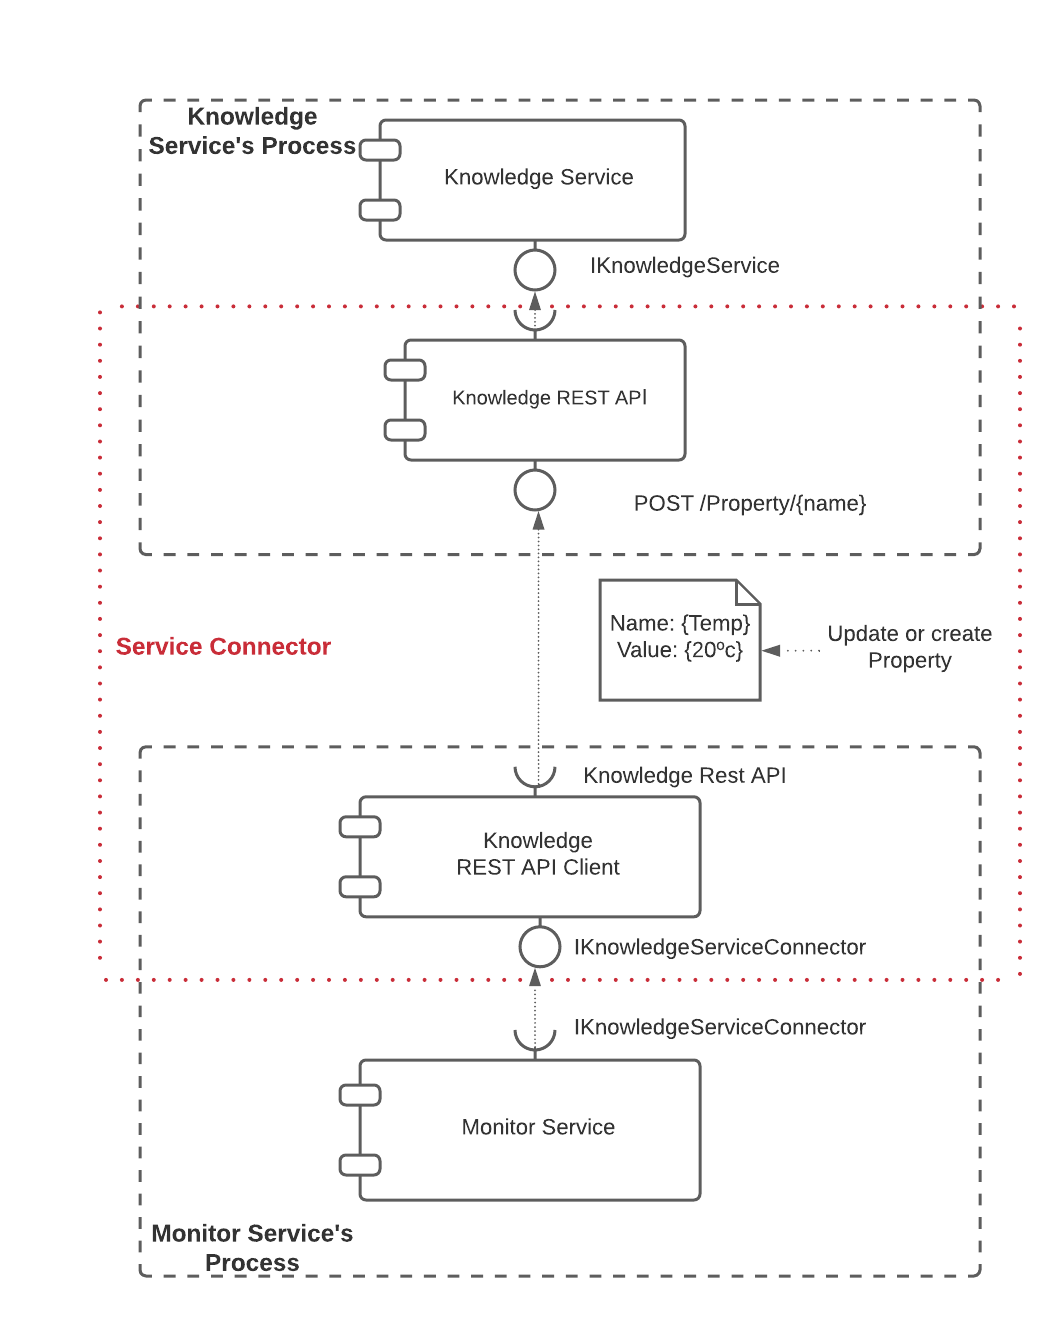
\includegraphics[scale=0.8]{02_arquitectura/images/Monitor-Knowledge-Connector}
  \caption{Diseño del conector usando implementación Cliente - Servidor}
  \label{fig:monitor-knowledge-connector-architecture}
\end{figure}

\subsection{Open API}
\label{chap:OpenAPI}

\begin{wrapfigure}{r}{0.35\linewidth}
  % \vspace{15pt}
  
\includegraphics[scale=0.34]{02_arquitectura/images/openapi-logo}
  \centering
  % \vspace{15pt}
\end{wrapfigure}

OpenAPI\footnote{Open API specification: \url{https://spec.openapis.org/oas/latest.html}} es un lenguaje estándar para describir APIs implementadas sobre el protocolo HTTP. Es un \textit{domain specific language} que podemos utilizar para describir APIs de nuestras aplicaciones

Para el desarrollo de este trabajo, hemos optado por utilizar conectores basados en APIs REST. Nos permitía utilizar mecanismos ya presentes en los microservicios que queríamos desarrollar, y que fueran más homogéneos.
Para facilitar la compatibilidad de los microservicios, y facilitar el desarrollo de nuevos microservicios, hemos decidido usar la especificación OpenAPI.

La principal ventaja que nos ofrecía OpenAPI era la posibilidad de generar código a partir de la especificación. Permite generar código tanto del cliente como del servidor. De esta forma, podíamos implementar nuestra API genérica en un lenguaje . En este caso, se decidió utilizar conjuntamente el lenguaje C\# junto con el framework ASP.NET Core, para implementar los microservicios iniciales.

A partir de estos microservicios, podemos exportar la especificación de OpenAPI, haciendo uso de los endpoints, atributos y comentarios. Por ejemplo, en este endpoint del servicio de monitorización, vemos cómo obtiene una propiedad del servicio de conocimiento.

Podemos observar cómo el método está decorado con atributos que describen el tipo de respuesta que produce, según el código de respuesta HTTP. Estos comentarios se utilizan en la generación de la especificación para obtener mejor implementación

Después, haciendo uso de las librerías de generación de código de OpenAPI.
